\chapter{Sampling, hypothesis testing, and the central limit theorem}

\section{The binomial distribution}

Let $X$ be the number of heads when a coin of bias $p$ is tossed $n$ times. 
The distribution of $X$ is so fundamental to probability and statistics that 
it merits a special name, the {\it binomial}($n,p$) distribution. Here it is,
precisely:
\begin{eqnarray*}
\Sigma     & = & \{0,1,\ldots, n\} \\
\pr(X = k) & = & {n \choose k} p^k (1-p)^{n-k}
\end{eqnarray*}
The figure below shows the binomial($100,0.6$) distribution.

\begin{center}
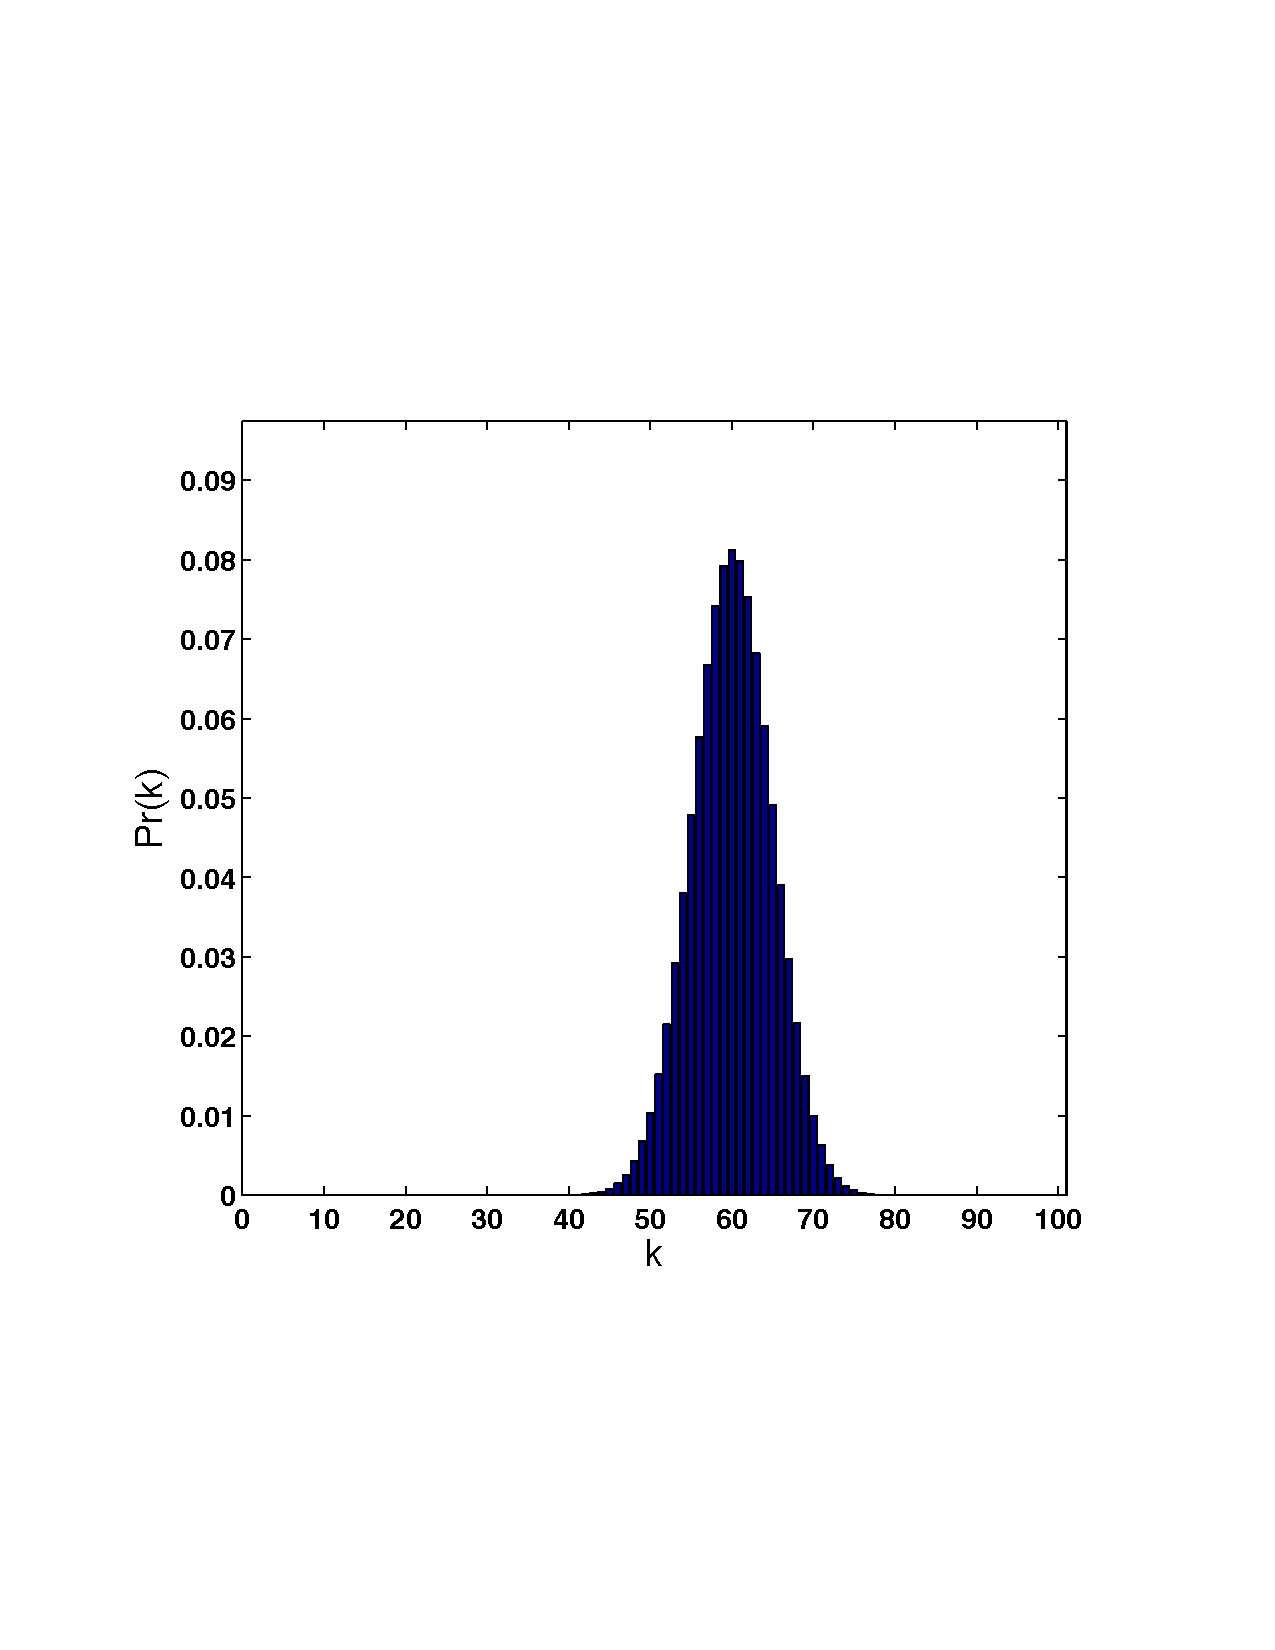
\includegraphics[width=3in]{figs/bin(100,06).pdf}
\end{center}

\noindent
The key property of this distribution is that it is tightly concentrated around
$np = 60$. This is the mean of $X$, as can be seen by writing it in the form
$X = X_1 + \cdots + X_n$, where each $X_i \sim B(p)$; in words, $X_i$ is 1 if
the $i$th coin toss comes up heads.

How spread out is the distribution? To quantify this, we need to compute the 
variance of $X$. Once again, the representation of $X$ as the sum of $X_i$'s
comes in handy, coupled with the following useful fact.
\begin{fact}
If $Z_1, \ldots, Z_n$ are independent, then 
$\var(Z_1 + \cdots + Z_n) = \var(Z_1) + \cdots + \var(Z_n)$.
\end{fact}
\noindent
Each $X_i$ has variance $p(1-p)$, so $X$ has variance $np(1-p)$ 
and thus standard deviation $\sqrt{np(1-p)}$.
\begin{fact}
If $X \sim \mbox{binomial}(n,p)$, then:
\begin{eqnarray*}
\E(X) & = & np \\
\var(X) & = & np(1-p) \\
\mbox{\rm stddev}(X) & = & \sqrt{np(1-p)}
\end{eqnarray*}
\end{fact}

There's another very useful fact about the binomial that comes up over and over again:
{\it about 95\% of the distribution lies within two standard deviations of the mean}.
That is to say,
\begin{equation}
\pr \left(np - 2 \sqrt{np(1-p)} \leq X \leq np + 2 \sqrt{np(1-p)}\right) 
\ \approx \ 0.95 . \label{eq:bin-2sigma}
\end{equation}
We'll see how this approximation arises a little later on. As an example of its use,
consider the figure shown above for binomial($100,0.6$). The standard deviation is 
$\sigma = \sqrt{100 (0.6) (0.4)} \approx 5$. And indeed almost all the 
distribution lies in the range $np \pm 2 \sigma = 60 \pm 10$.

The remarkable thing about (\ref{eq:bin-2sigma}) is that although $X$ can potentially
take on $n+1$ possible values, it effectively stays within a range of size just 
$O(\sqrt{n})$; this is miniscule compared to $n+1$ for large $n$.

\section{Hypothesis testing}

\subsection{Testing a vaccine}

Suppose there is a certain disease that cattle can contract; and that any given 
cow has a 25\% chance of contracting it within the course of a year. A new serum 
is proposed, and we want to test it to see how well it works. So we choose $n$ cows 
at random, inject them with the serum, and then keep an eye on them over the next 
year. Let's say $K$ of them remain healthy.

One possibility is that the serum has no effect whatsoever; call this hypothesis 
$H_0$. If this hypothesis is true, then the chance of infection is exactly the 
same for the cows that were injected as it is for the cow population at large, 
and thus $K \sim \mbox{binomial}(n,0.75)$.

We hope that the experiment yields a large value of $K$; this will provide evidence
against hypothesis $H_0$. But how large does $K$ need to be? It depends on how much
{\it statistical confidence} we want in our assertion that $H_0$ is false. A common
goal is a {\it 95\% confidence level}.

Suppose we have a sample of $n=100$ cows. The binomial($100,0.75$) distribution has 
mean $75$ and standard deviation $\sigma = \sqrt{100(0.25)(0.75)} \approx 4.3$. 
Using equation (\ref{eq:bin-2sigma}), we can deduce that {\it if $H_0$ were true}, 
we would expect (with 95\% confidence) a value of $K$ in the range $75 \pm 8.6$. 
If $K$ exceeds this, that is if $K > 83$, then we can reject $H_0$ with a 95\% 
confidence level.

\subsection{A blood pressure drug}

Suppose a new blood pressure drug is proposed, and to test it, a sample of
$n$ patients is selected. Their blood pressure is measured with and without
the drug.

\begin{tabular}{ccc}
Person   & B.P. with drug & B.P. without drug \\
1        & $x_1$          & $x_1'$ \\
2        & $x_2$          & $x_2'$ \\
$\vdots$ & $\vdots$       & $\vdots$ \\
$n$      & $x_n$          & $x_n'$
\end{tabular}

\noindent
The $i$th trial is called a success if $x_i < x_i'$; let $K$ be the total number
of successes. How should the evidence be evaluated?

Let $H_0$ be the hypothesis that the drug is useless. Under this hypothesis,
$K \sim \mbox{binomial}(n,0.5)$. Thus $K$ has expected value $0.5 n$ and 
standard deviation $\sqrt{n (0.5) (0.5)} = 0.5 \sqrt{n}$. As we
noted above, with 95\% confidence, we'd expect $K$ to be within two standard
deviations of its mean, that is, $K = 0.5 n \pm \sqrt{n}$.

So if $K$ exceeds $0.5n + \sqrt{n}$, we can declare that $H_0$ is invalidated
with 95\% confidence, implying that the drug is not entirely useless.

\section{Sampling}

We live in an age where the government and the mass media are continuously polling
the public. They wish to know the fraction of people who like sushi, think Obama
is doing a good job, support Tiger Woods, think God exists, feel pessimistic
about the future, smoke, think the war in Iraq is unnecessary, etc. This constant
polling affects decision-making at every level. It advises politicians on what to
say and do. It helps companies decide how to most effectively advertise their
products. It helps investors decide where to entrust their money. And so on.

In each such case, there is an unknown probability $p$ that is sought: the fraction
of people who like sushi, for instance. Determining this fraction exactly would
require asking {\it everyone}, which is prohibitively expensive. So instead a
sample of $n$ people is chosen at random, and they are each asked whether they
like sushi. Let $K$ be the number of positive responses. Then $K$ has the
binomial($n,p$) distribution, with expected value $np$ and variance $np(1-p)$.

An estimate of the fraction of sushi-lovers is $K/n$. Notice that
\begin{eqnarray*}
\E\left(\frac{K}{n}\right) & = & p \\
\var\left(\frac{K}{n} \right) & = & \frac{\var(K)}{n^2} \ \ = \ \ \frac{p(1-p)}{n} \\
\mbox{stddev}\left(\frac{K}{n}\right) & = & \sqrt{\frac{p(1-p)}{n}}
\end{eqnarray*}
A standard rule of thumb, given in equation (\ref{eq:bin-2sigma}) is that the 
estimate $K/n$ will lie within two standard deviations of its expected value 
with 95\% probability. Thus we can assert with 95\% confidence that the true 
fraction of people who like sushi is 
$$ \frac{K}{n} \pm 2 \sqrt{\frac{p(1-p)}{n}} .$$
But this doesn't make sense, since we don't know what $p$ is. A quick fix is
to notice that $p(1-p) \leq 1/4$ (the maximization can be done by calculus,
for instance), and thus a valid 95\% confidence interval is
$$ \frac{K}{n} \pm \frac{1}{\sqrt{n}} .$$
Thus a sample size of $2{,}500$ gives an estimate that is accurate to within
$1/\sqrt{n} = 0.02$ (at 95\% confidence), whereas a sample size of $10{,}000$
gives an accuracy of $0.01$.

What if we want a higher level of confidence, like 99\%, or even 99.9\%?
Equation (\ref{eq:bin-2sigma}) is no longer helpful; we need similar 
approximations for other confidence levels. It turns out that these are
easy to obtain, for any desired confidence level, using the {\it normal
approximation to the binomial distribution}.

{\bf read up to here for Wed 11/16}
\section{The normal distribution}

You are probably reading these notes in a library or cafeteria. Take a look
at the 100 or so people nearest to you. If you were to plot the heights of 
all the men, it would look kind of like this:

\begin{center}
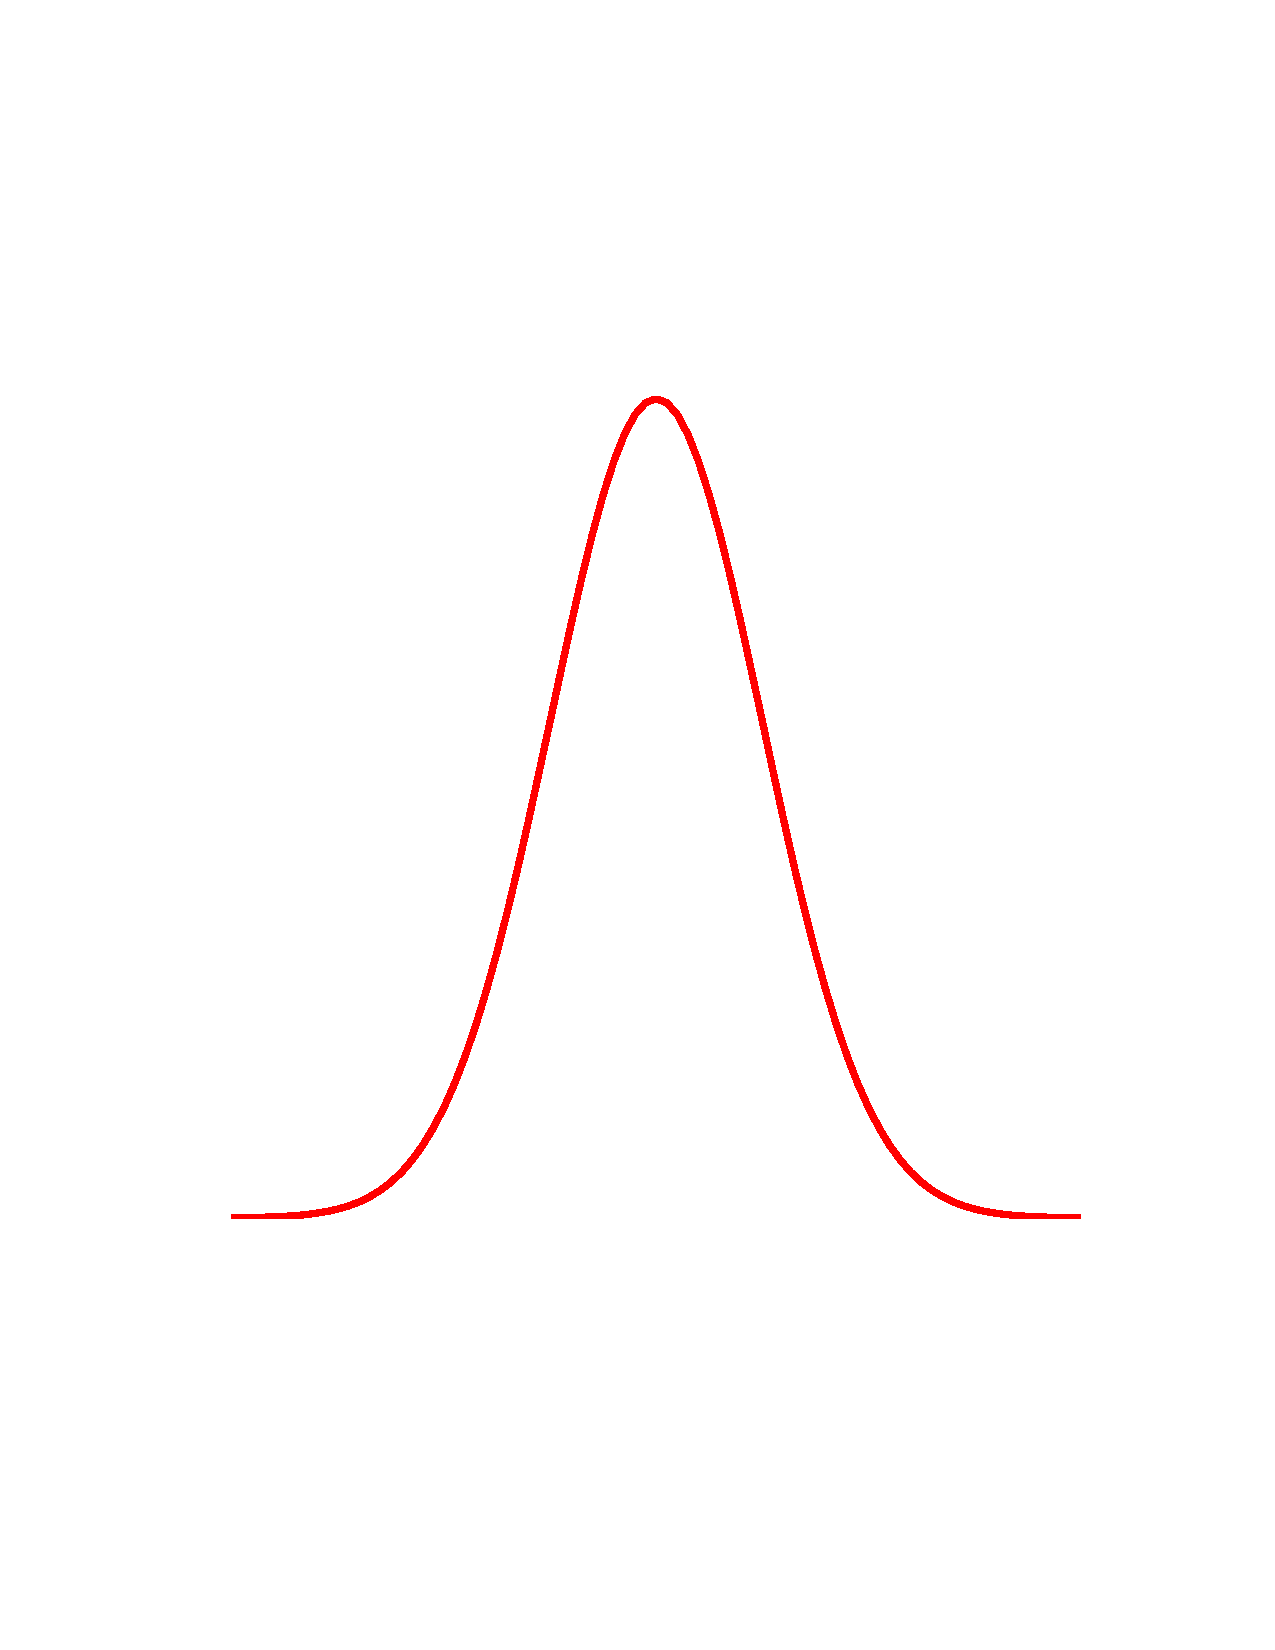
\includegraphics[width=3in,height=1.5in]{figs/bell.pdf}
\end{center}

\noindent
If you were to plot the blood pressure of all the women, it would look much 
the same. Or if you plotted the velocities of the molecules in the air, once 
again, same thing. This one distribution is everywhere. For that reason it 
is called the {\it normal} distribution.

The normal distribution with mean $\mu$ and variance $\sigma^2$ is denoted
$N(\mu, \sigma^2)$. Unlike most of the examples we've seen so far, it is
a {\it continuous} distribution, a density over the real line. The density 
at any point $x$ is
$$ \frac{1}{\sigma \sqrt{2\pi}} e^{-(x-\mu)^2/2\sigma^2} .$$
Don't worry too much about this specific functional form. Instead, let's
look at pictures of three different normal distributions.

\begin{center}
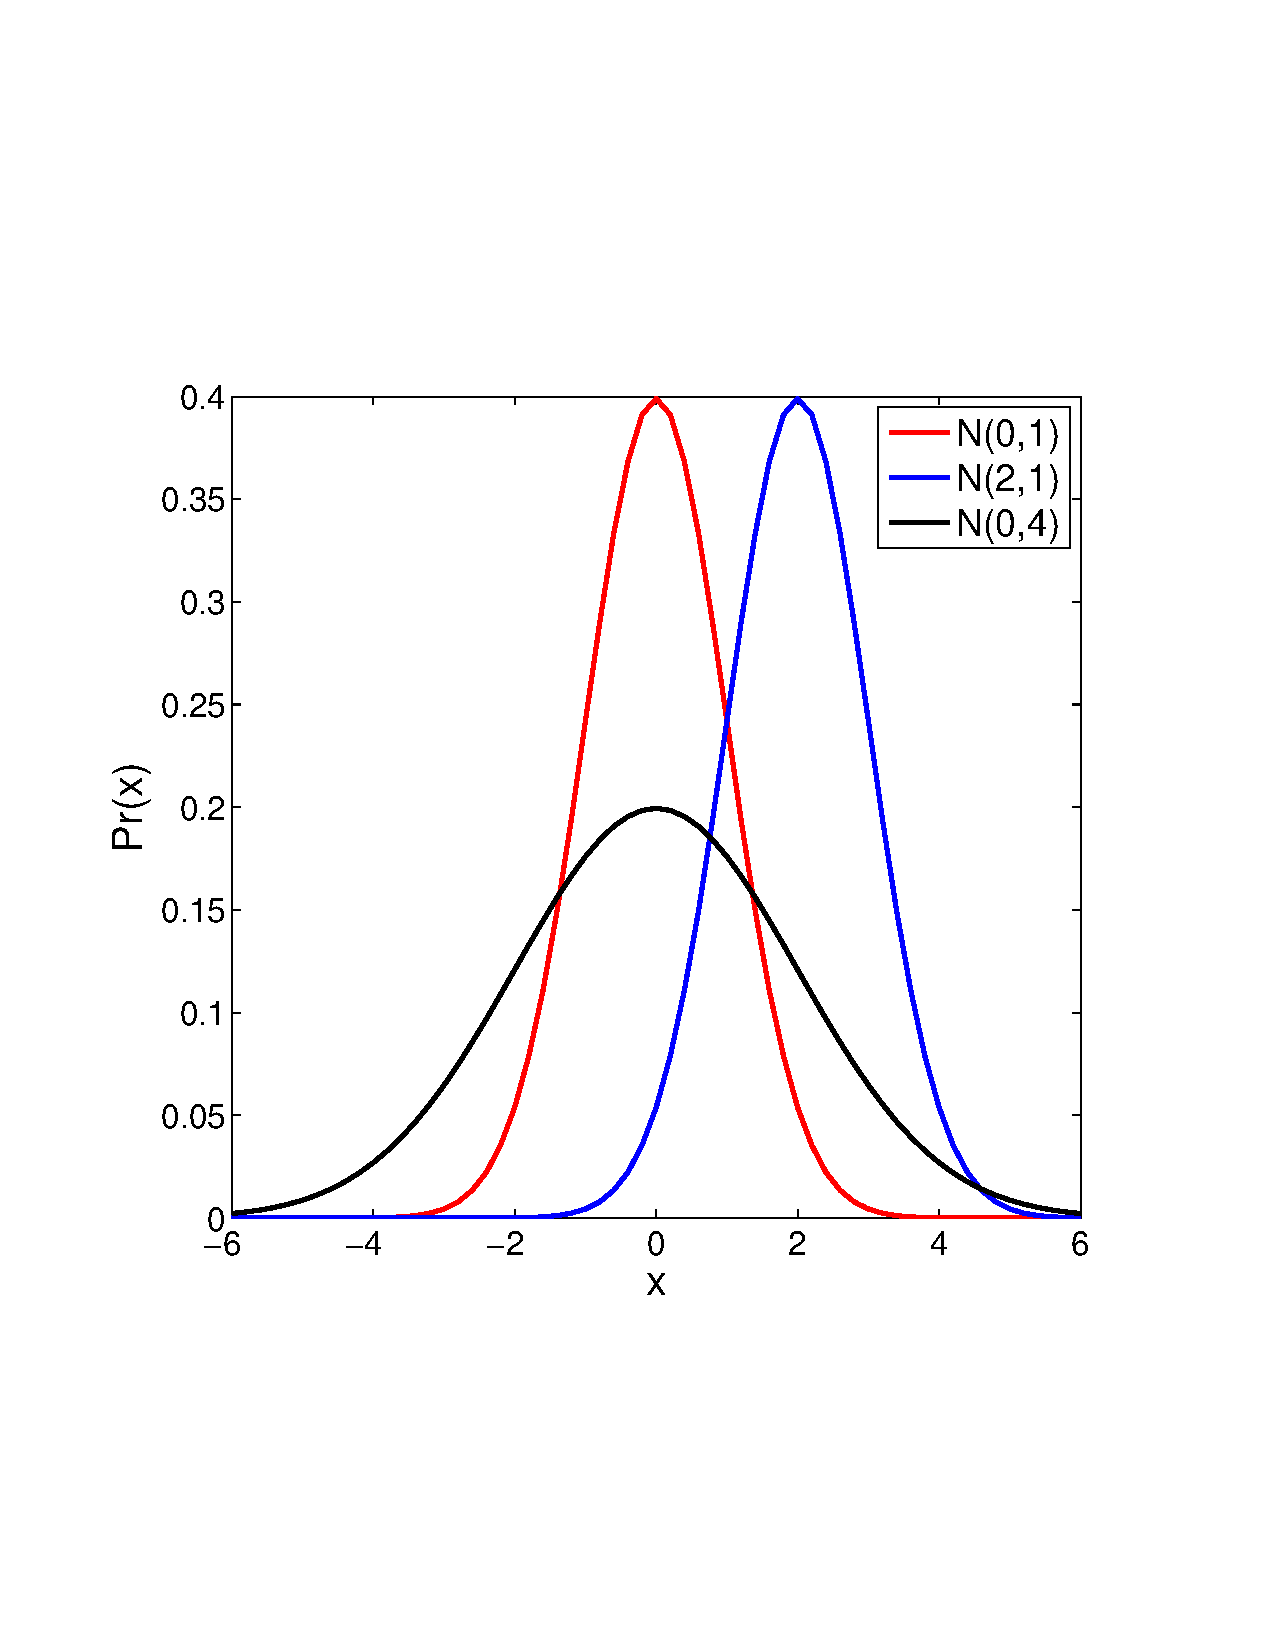
\includegraphics[width=4in,height=3in]{figs/three-norm.pdf}
\end{center}

\noindent
The red curve (or, if you're reading this in black and white, the tall curve
in the middle) is $N(0,1)$: the normal distribution with mean 0 and
variance 1. This is sometimes called the {\it standard normal}. All other
normal distributions are simply scaled and translated versions of it. For
instance, the blue curve (the one on the right) is $N(2,1)$, which is obtained
by shifting the standard normal two units to the right. The black curve (the
wide one in the middle), on the other hand, is $N(0,4)$, obtained by scaling
the standard normal by a factor of two. Here's a summary of the relationship 
between different normal distributions.
\begin{fact}
If $X \sim N(\mu, \sigma^2)$ then $aX + b \sim N(a\mu + b, a^2 \sigma^2)$.
\end{fact}

\subsection{Sums of independent random variables}

Here's an interesting fact about the normal distribution.
\begin{fact}
If $X,Y$ are independent, with $X \sim N(\mu_1, \sigma_1^2)$ and 
$Y \sim N(\mu_2, \sigma_2^2)$, then $X + Y \sim N(\mu_1+\mu_2, \sigma_1^2+ \sigma_2^2)$.
\end{fact}
In words, if a bunch of independent random variables are each normally distributed, 
and you add them up, the result still has a normal distribution.

In fact, something much more spectacular is true: even if the independent random 
variables are {\it not} normally distributed, their sum looks like a normal 
distribution! 
\begin{fact}[Central limit theorem]
Suppose $X_1, \ldots, X_n$ are independent with mean $\mu$ and variance $\sigma^2$.
Then for sufficiently large $n$, the distribution of $(X_1 + \cdots + X_n)/n$ is
approximately $N(\mu, \sigma^2/n)$. Equivalently, the distribution of 
$X_1 + \cdots + X_n$ is approximately $N(n \mu, n \sigma^2)$.
\end{fact}
This astonishing fact helps explain why the normal distribution is observed all
over the place.

\subsection{Tails of the normal}

In sampling and hypothesis testing, we ultimately end up adding independent random
variables; more on this below. Thus the result is well-approximated by the normal
distribution, and by analyzing the tails of this distribution, we can get 
intervals for any desired level of confidence.

Suppose $X \sim N(\mu,\sigma^2)$. If we want a 95\% confidence interval, we seek a 
value of $z$ for which 
$$ \pr(\mu-z \leq X \leq \mu+z) = 0.95 .$$
The answer, it turns out, is $z = 2 \sigma$. If we want a 99\% confidence interval, we
seek a value of $z$ for which
$$ \pr(\mu-z \leq X \leq \mu+z) = 0.99 .$$
In this case, $z = 3 \sigma$.

Here is a summary of some key facts about tails of the normal.
\begin{fact}
If $X \sim N(\mu, \sigma^2)$, then:
\begin{itemize}
\item With 66\% probability, $X$ lies between $\mu-\sigma$ and $\mu+\sigma$.
\item With 95\% probability, $X$ lies between $\mu-2\sigma$ and $\mu+2\sigma$.
\item With 99\% probability, $X$ lies between $\mu-3\sigma$ and $\mu+3\sigma$.
\end{itemize}
\label{fact:normal-tails}
\end{fact}

\section{Sampling revisited}

\subsection{Polls with yes/no answers}

From the population at large $n$ people are chosen at random and are asked a particular
question (``Do you approve of the corporate bailouts?''). The goal is to estimate 
the fraction $p$ of the underlying population that would answer yes. Let's say
that $K$ of the sampled people say yes; then $K \sim \mbox{binomial}(n,p)$, and
thus a reasonable estimate of $p$ is $K/n$.

To analyze the situation further, it helps to approximate the binomial by a normal
distribution. Notice that 
$$ K = X_1 + X_2 + \cdots + X_n $$
where the $X_i$ are independent $B(p)$ random variables (``did the $i$th person 
say yes?''). By the central limit theorem,
$$ \frac{K}{n} \mbox{\ is distributed like\ } N\left( p, \ \frac{p(1-p)}{n} \right) .$$
Writing $\sigma = \sqrt{\frac{p(1-p)}{n}} \leq \frac{1}{2\sqrt{n}}$, we can conclude from 
Fact~\ref{fact:normal-tails} that the estimate $K/n$ is accurate within
\begin{itemize}
\item $\frac{1}{2\sqrt{n}}$ with at least 66\% probability.
\item $\frac{1}{\sqrt{n}}$ with at least 95\% probability.
\item $\frac{3}{2\sqrt{n}}$ with at least 99\% probability.
\end{itemize}
And other confidence intervals are also easy to obtain, from standard tables of 
the normal distribution.
 
\subsection{Polls with numeric answers}

Many polls demand numeric rather than yes/no answers. How many glasses of wine do
you drink daily? What is your salary? How old are you? And so on.

Suppose, for instance, that we wish to assess the overall educational levels
(number of years of schooling) of residents of San Diego. If we were to consider 
{\it all} San Diegans of age $\geq 25$, this would be a distribution with some 
unknown mean $\mu$ and standard deviation $\sigma$. We would like to estimate 
$\mu$, the average educational level. So we randomly pick $n$ people of age 
$\geq 25$ and ask them how many years they have spent in school. Suppose their 
answers are $X_1, \ldots, X_n$.

The empirical mean (the mean of the samples) is
$$ M \ = \ \frac{X_1 + \cdots + X_n}{n} $$
and the empirical standard deviation is
$$ S \ = \ \sqrt{\frac{(X_1 - M)^2 + \cdots + (X_n - M)^2}{n}} .$$
It is reasonable to use $M$ as an estimate of $\mu$. What kind of confidence
interval can we give for it?

This is where the central limit theorem once again comes in. Since the $X_i$ are
independent, we can assert that
$$ M \mbox{\ is distributed like\ } N\left(\mu, \frac{\sigma^2}{n} \right) .$$
Thus we immediately have the following confidence intervals, from 
Fact~\ref{fact:normal-tails}.
\begin{itemize}
\item With 95\% probability, $M$ is lies between $\mu-\frac{2\sigma}{\sqrt{n}}$ and 
$\mu+\frac{2\sigma}{\sqrt{n}}$.
\item With 99\% probability, $M$ lies between $\mu-\frac{3\sigma}{\sqrt{n}}$ and 
$\mu+\frac{3\sigma}{\sqrt{n}}$.
\end{itemize}
Thus, for instance, when using $M$ to estimate $\mu$, we can be 95\% certain that 
it is accurate within $\pm \frac{2\sigma}{\sqrt{n}}$. But wait: we don't know
$\sigma$. So instead, it is customary to use the empirical standard deviation
instead, and to assert that $M$ is accurate within  $\pm \frac{2 S}{\sqrt{n}}$,
with 95\% confidence.

Returning to the schooling example, suppose we poll $n = 400$ people, and find 
that the empirical average and standard deviation are $M = 11.6$ and $S = 4.1$,
respectively. Then we can assert with 95\% confidence that the average number
of years of schooling of San Diegans is
$$ 11.6 \pm \frac{2 \times 4.1}{\sqrt{400}} \ \ = \ \ 11.6 \pm 0.41 .$$

 
\section{The Bonferroni correction}
When performing statistical test, we often want to use the same data
set to test many different alternative hypotheses. For example, when
studying high blood pressure we might want to support or refute
the following hypotheses
\begin{enumerate}
\item Blood pressure is elevated in patients with high cholesterol.
\item Blood pressure is elevated in older patients.
\item High blood pressure is caused by stress.
\item Blood pressure is elevated in patients that eat too many
  vegetables.
\item and so on.
\end{enumerate}
Suppose we run a test whose significance is $\alpha$ for each of these
hypotheses and find that one of the tests rejects the null
hypothesis. Can we say that the significance of this rejection is
$\alpha$? Clearly, as the number of tests increases, the significance
of each test decreases. How can we account for that? It is tempting to
think of passing each test as an independent event and calculate the
overall significance based on that. However, we don't know whether the
tests are independent or not. In fact, the opposite is probably true:
older patients tend to also have high cholesterol.

We therefor do the safe thing and use the union bound. Let $T_i$,
$i=1,\ldots,n$ be the event corresponding to test $i$ rejecting the
null hypothesis when the null hypothesis is in fact true. Suppose that
the $p$ value of each of the $n$ tests is at most $\alpha$,
i.e. $P(T_i) \leq \alpha$.
 
The union bound tells us that 
\[
P\left( \bigcup_{i=1}^n T_i \right) \leq \sum_{i=1}^n P(T_i) \leq n \alpha
\]

\section{Estimating the size of large populations}
Statistical techniques are useful for estimating the size of a large
population. Suppose for example that we want to count the number of
fish in a lake. How would we do that? Instead of trying to catch all
the fish, which is both impossible and damaging to the fish
population, we perform the following two phase test:
\begin{enumerate}
\item We catch fish, mark them with some non-intrusive marker, and
  release them back to the lake. Suppose we mark $m$ of them with a
  mark that sticks to the fish but does not hurt it.
\item After we marked the $m$ fish, we wait for them to mix with the
  other fish and then catch $l$ fish and count how many of these
  have been marked. We denote the number of marked fish by the random
  variable $Y$.
\end{enumerate}
The probability that each that each fish caught in the second batch is
marked is equal to the fraction of all of the fish in the lake that
are marked, which is $m/n$. This means that the random variable $Y$ is
a sum of $l$ independent binary random variables each with mean $m/n$.
Therefor the mean of $Y$ is $(lm)/n$. The standard deviation of each
of the binary variables is at most $1/2$ (which happens when
$m/n=1/2$). Thus the standard deviation of $Y$ is $\sqrt{l}/2$.
Therefor the 95\% significance interval for $(lm)/n$ is
$[Y-\sqrt{l},Y+\sqrt{l}]$.

We are interested in estimating $n$, therefor our estimate is the range.
\[
\left[\frac{lm}{Y+\sqrt{l}}, \frac{lm}{Y-\sqrt{l}} \right]
\]

Note that if the number of fish in the lake $n$ is large, so that $m/n
\approx 1/l$ then there is a good chance we will see no marked fish in
the second batch. We might need to mark more and more fish until the
chance of catching a marked fish becomes reasonably high.

